\documentclass[12pt]{report}
\usepackage{tikz}
\begin{document}
%general formula: \draw[parameters] (x, y) <SHAPE TYPE> (parameters)
% here's a basic drawing with lines and simple shapes 
\begin{tikzpicture}
\draw (0,0) -- (4,0) -- (4,4) -- (0,4) -- (0,0);
\draw (1,-1) -- (5,-1) -- (5,3) -- (1,3) -- cycle;
%rectangles specify lower left and upper right 
\draw (0,0) rectangle (6,6);
\draw (0,0) parabola (4,4);
\end{tikzpicture}

\vspace{5em}
%more shapes 
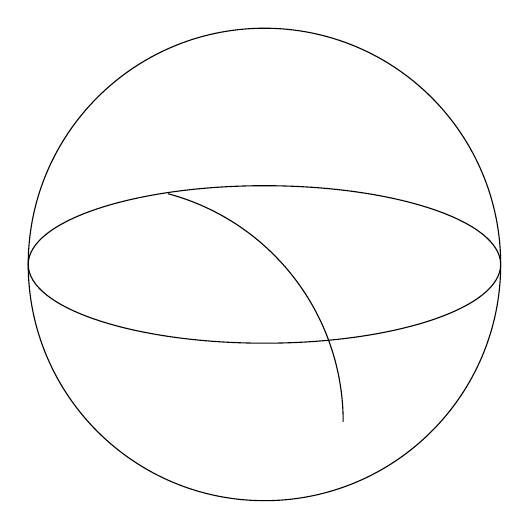
\begin{tikzpicture}
\draw (2,2) circle (3cm);
\draw (2,2) ellipse (3cm and 1cm);
\draw (3,0) arc (0:75:3cm);
\end{tikzpicture}

\vspace{5em}
%using parameters 
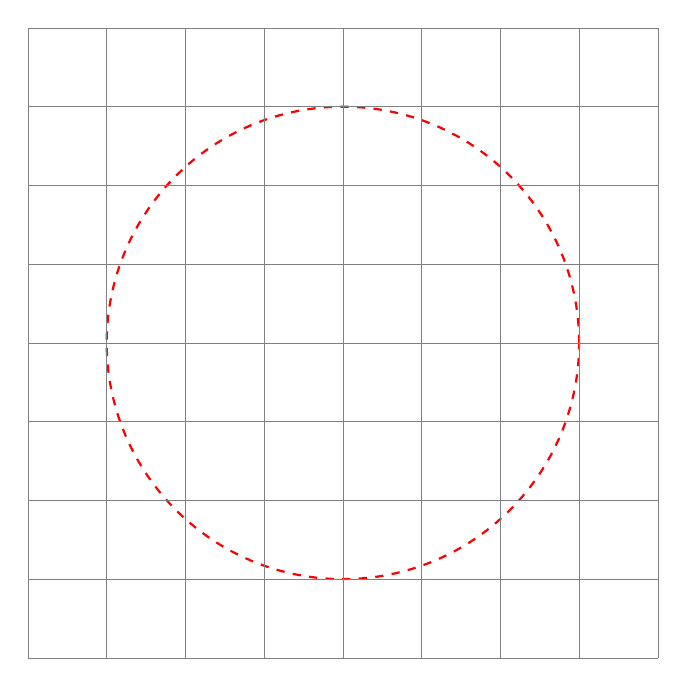
\begin{tikzpicture}
\draw[red,thick,dashed] (2,2) circle (3cm);
\draw[step=1cm,gray,very thin] (-2,-2) grid (6,6);
\end{tikzpicture}

\vspace{5em}
%using fill and shade commands
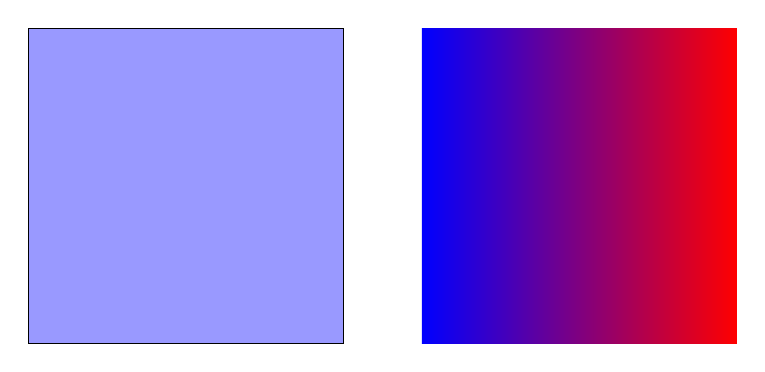
\begin{tikzpicture}
\fill[blue!40!white, draw=black] (0,0) rectangle (4,4);
\shade[left color=blue,right color=red] (5,0) rectangle (9,4);
\end{tikzpicture}

\begin{center}
\begin{tikzpicture}
    \node[shape=circle,draw=black] (B) at (0,0) {B};
    \node[shape=circle,draw=black] (A) at (1.5,3) {A};
    \node[shape=circle,draw=black] (C) at (3,0) {C};
    \node[shape=circle,draw=black] (D) at (1.5, -3) {D};
    \path [->] (B) edge node[left] {} (A);
    \path [->](B) edge node[left] {} (C);
    \path [->](D) edge node[left] {} (C);
\end{tikzpicture}
\end{center}
\end{document}